\documentclass[12pt]{scrartcl}
\usepackage[hidelinks]{hyperref}
\usepackage[utf8]{inputenc}
\usepackage[square]{natbib}
\usepackage{graphicx}
\usepackage{minted}
\usepackage{subcaption}

\title{Towards Parallel Detection of Movement Patterns in Large Spatio-temporal Datasets}
\author{Andres Oswaldo Calderon Romero}

\begin{document}

\maketitle
 
\section{Introduction}
Nowadays, spatio-temporal data is ubiquitous. Thanks to new technologies and the proliferation of location devices (such as Internet of Things, Remote Sensing, Smart phones, GPS, RFID, etc.), the collection of huge amount of spatio-temporal data is now possible. With the appearance of this datasets also appears the need of new techniques which allow the analysis and detection of useful patterns in large spatio-temporal databases.  

Applications for this kind of information are diverse and interesting, in particular if they come in the way of trajectory datasets \citep{jeung_trajectory_2011, huang_mining_2015}. Case of studies range from transportation system management \citep{di_lorenzo_allaboard:_2016,johansson_efficiency_2015} to Ecology \citep{johnston_abundance_2015, la_sorte_convergence_2016}.  For instance, \cite{turdukulov_visual_2014} explore the finding of complex motion patterns to discover similarities between tropical cyclone paths.  Similarly, \cite{amor_persistence_2016} use eye trajectories to understand which strategies people use during a visual search. Also, \cite{holland_movements_1999} track the behavior of tiger sharks in the coasts of Hawaii in order to understand their migration patters.

Recently, there has been an increasing interest in exploiting more complex movement patterns in spatio-temporal datasets.  Traditional range and nearest neighbor queries do not capture the collective behavior of moving objects.  Moving cluster \citep{kalnis_discovering_2005}, convoys \citep{jeung_discovery_2008} and flock patterns \citep{benkert_reporting_2008, gudmundsson_computing_2006} are new movement patterns which unveil how entities move together during a minimum time interval.  

In particular, a moving flock pattern show how objects move close enough during a given period of time.  A better understanding on how entities move in space is of special interest in areas such as sports \citep{iwase_tracking_2002},  surveillance and security \citep{makris_path_2002,piciarelli_trajectory_2005}, urban development \citep{huang_trajgraph:_2016, long_combining_2015} and socio-economic geography \citep{frank_life_2000}.

Despite the fact that much more data become available, state-of-the-art techniques to mine complex movement patterns still depict low scalability and poor performance in big spatial data.  The present work aims to find an initial solution to implement a parallel method to discover moving flock patterns in large spatio-temporal datasets.  It is thought that new trends in distributed in-memory framework for spatial operations could help to speed up the detection of this kind of patterns.

The following section will state the related work in the area.  Section \ref{sec:candidates} will explain the details of the implementation of the proposed solution while section \ref{sec:experiments} will present their experimental results. Finally, section \ref{sec:conclusions} will discuss some conclusions and future work. 

\section{Related work}
Recently increase use of location-aware devices (such as GPS, Smart phones and RFID tags) has allowed the collection of a vast amount of data with a spatial and temporal component linked to them.  Different studies have focused in analyzing and mining this kind of collections \citep{leung_knowledge_2010, miller_geographic_2001}.  In this area, trajectory datasets have emerged as an interesting field where diverse kind of patterns can be identified \citep{zheng_computing_2011, vieira_spatio-temporal_2013}.  For instance, authors have proposed techniques to discover motion spatial patterns such as moving clusters \citep{kalnis_discovering_2005}, convoys \citep{jeung_discovery_2008} and flocks \citep{benkert_reporting_2008, gudmundsson_computing_2006}.  In particular, \cite{vieira_-line_2009} proposed BFE (Basic Flock Evaluation), a novel algorithm to find moving flock patterns in polynomial time over large spatio-temporal datasets.  
 
A flock pattern is defined as a group of entities which move together for a defined lapse of time \citep{benkert_reporting_2008} (figure \ref{fig:flock}).  Applications to this kind of patterns are rich and diverse.  For example, \citep{calderon_romero_mining_2011} finds moving flock patterns in iceberg trajectories to understand their movement behavior and how they related to changes in ocean's currents. 

\begin{figure}
 \centering
 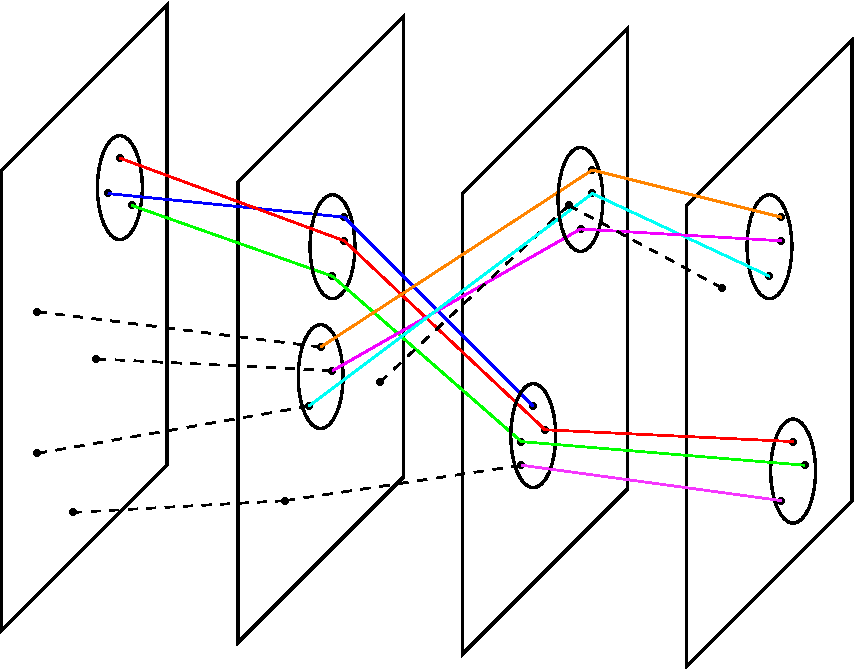
\includegraphics[width=0.5\textwidth]{./figures/flock}
 \caption{Moving flock pattern example.}
 \label{fig:flock}
\end{figure}
 
The BFE algorithm presents an initial strategy in order to detect flock patterns.  In that, first it finds disks with a predefined diameter ($\varepsilon$) where moving entities could be close enough at a given time interval.  This is a costly operation due to the large number of points and intervals to be analyzed ($\mathcal{O}(2n^2)$ per time interval).  The technique uses a grid-based index and a stencil (see figure \ref{fig:grid}) to speed up the process, but the complexity is still high.

\cite{calderon_romero_mining_2011} and \cite{turdukulov_visual_2014} use a frequent pattern mining approach to improve performance during the combination of disks between time intervals.  Similarly, \cite{tanaka_improved_2016} introduce the use of plane sweeping along with binary signatures and inverted indexes to speedup the same process.  However, the above-mentioned methods still keep the same strategy as BFE to find the disks at each interval.  

\cite{arimura_finding_2014} and \cite{geng_enumeration_2014} use depth-first algorithms to analyze the time intervals of each trajectory to report maximal duration flocks.  However, these techniques are not suitable to find patterns in an on-line fashion.

Given the high complexity of the task, it should not be surprising the use of parallelism to increase performance.  \cite{fort_parallel_2014} use extreme and intersection sets to report maximal, longest and largest flocks on the GPU with the limitations of its memory model.  

Indeed, despite the popularity of cluster computing frameworks (in particular whose supporting spatial capabilities \citep{eldawy_spatialhadoop:_2014, yu_demonstration_2016, pellechia_geomesa:_2015-1, xie_simba:_2016-1}) there are not significant advances in this area.  At the best of our knowledge, this work is the first to explore in-memory distributed systems towards the detection of moving flock patterns.

\begin{figure}
 \centering
 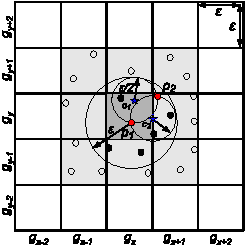
\includegraphics[width=0.3\textwidth]{./figures/grid}
 \caption{Grid-based index used in \cite{vieira_-line_2009}.}
 \label{fig:grid}
\end{figure}

\section{Parallelizing candidate disk detection}\label{sec:candidates}

Given that the finding of disks at each time interval is one of the most costly operations towards the detection of moving flock patterns, the main goal of this work is to implement a parallel method to detect that set of disks.  In order to do that, we will use the spatial operations offered by Simba \citep{xie_simba:_2016-1}, a distributed in-memory spatial analytic engine based on Apache Spark. This section explains the details of the algorithm implemented in Simba and how some spatial predicates introduced by it can leverage the finding of disks.

\subsection{Spatial operations on Simba}
Simba (Spatial In-Memory Big data Analytics) extends the Spark SQL engine to provide rich spatial operations through both SQL and the DataFrame API.  Besides, it introduces two-layer spatial indexing and cost-based optimizations to support efficient spatial queries in parallel.  Simba is open source and public available at the project's website\footnote{\url{http://www.cs.utah.edu/~dongx/simba/}}.

In particular, \texttt{DISTANCE JOIN} and \texttt{CIRCLERANGE} operators were used in order to find groups of points lying close enough each other.  The algorithm uses a user-defined distance ($\varepsilon$) to define the diameter of the disk.  Figure \ref{fig:sql} shows the SQL statement used to find pairs of points inside an $\varepsilon$ distance in parallel.

\begin{figure}
 \centering
    \begin{minted}[fontsize=\footnotesize,tabsize=8,breaklines,framesep=10pt,frame=single, escapeinside=||,mathescape=true]{sql}
SELECT 
	* 
FROM 
	points p1
|\color{blue}{DISTANCE JOIN}|
	points p2 
ON 
	POINT(p2.x, p2.y) IN |\color{blue}{CIRCLERANGE}|(POINT(p1.x, p1.y), |$\varepsilon$|)
WHERE 
	p1.id < p2.id
    \end{minted}
 \caption{SQL statement on Simba to find points lying inside an $\varepsilon$ distance.}
 \label{fig:sql}
\end{figure}

\subsection{Finding disks for pairs of points}
Once the set of pairs of points has been found, a map function computes the center of the two possible disks per each pair according to the BFE algorithm.  \cite{vieira_-line_2009} states that:  ``For each such pair there are exactly two disks with radius $\frac{\varepsilon}{2}$ that have those points on their circumference''.  Figure \ref{fig:theorem} illustrates how to find the center of those disks.

\begin{figure}
 \centering
 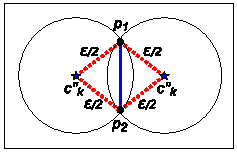
\includegraphics[width=0.4\textwidth]{figures/theorem} 
 \caption{Disks for $\{p_1,p_2\},\ d(p_1,p_2) \leq \varepsilon$ \citep{vieira_-line_2009}.}
 \label{fig:theorem}
\end{figure}

After that, the complete set of candidate disks is collected and ready to be processed by the following phases of the BFE algorithm. 

The implementation of the proposed method was written in Scala 2.10.6 and tested in Simba/Spark 1.6.0.  The current code can be accessed at the authors' repository\footnote{ \url{https://github.com/aocalderon/PhD/tree/master/Y2Q1/SDB/Project/Code/Scripts/pbfe2}}.

\subsection{Experiments}\label{sec:experiments}
The main idea of the experiments is to assess the performance of the parallel method against a sequential version of the BFE algorithm proposed by \cite{vieira_-line_2009}.  A public available implementation written in Python can be accessed at this repository\footnote{\url{https://github.com/poldrosky/FPFlock}}.  The source code was modified to stop after the finding of the disks and report the total number of computed disks.  Same configuration was followed by the parallel implementation.

Next, a set of experiments evaluates the execution time of both algorithms on two real datasets.  Further details of the settings and datasets are discussed below.

\subsection{Beijing dataset}
This dataset was extracted from the Geolife project\footnote{\url{https://www.microsoft.com/en-us/download/details.aspx?id=52367}} \citep{zheng_understanding_2008, zheng_mining_2009, zheng_geolife:_2010}.  It collects GPS trajectories of 182 users in a period of over three years (from April 2007 to August 2012) for an overall total of 17,621 trajectories.  The timestamp field was ignored and duplicate locations were removed to simulate an unique and large time interval.  In total, the point dataset contains $\approx$18 million points.

An initial set of experiments takes relatively small samples of the data and runs the algorithms under different values of $\varepsilon$. Experiments were deployed in a single-node machine with a 4-core Intel(R) Core(TM) i5-2400S CPU @ 2.50GHz processor, 8 GB of RAM running Ubuntu 16.04 LTS, Python 3.5 and Simba/Spark 1.6.0.  Figure \ref{fig:beijing} show the results of these experiments.

\begin{figure}
 \centering
 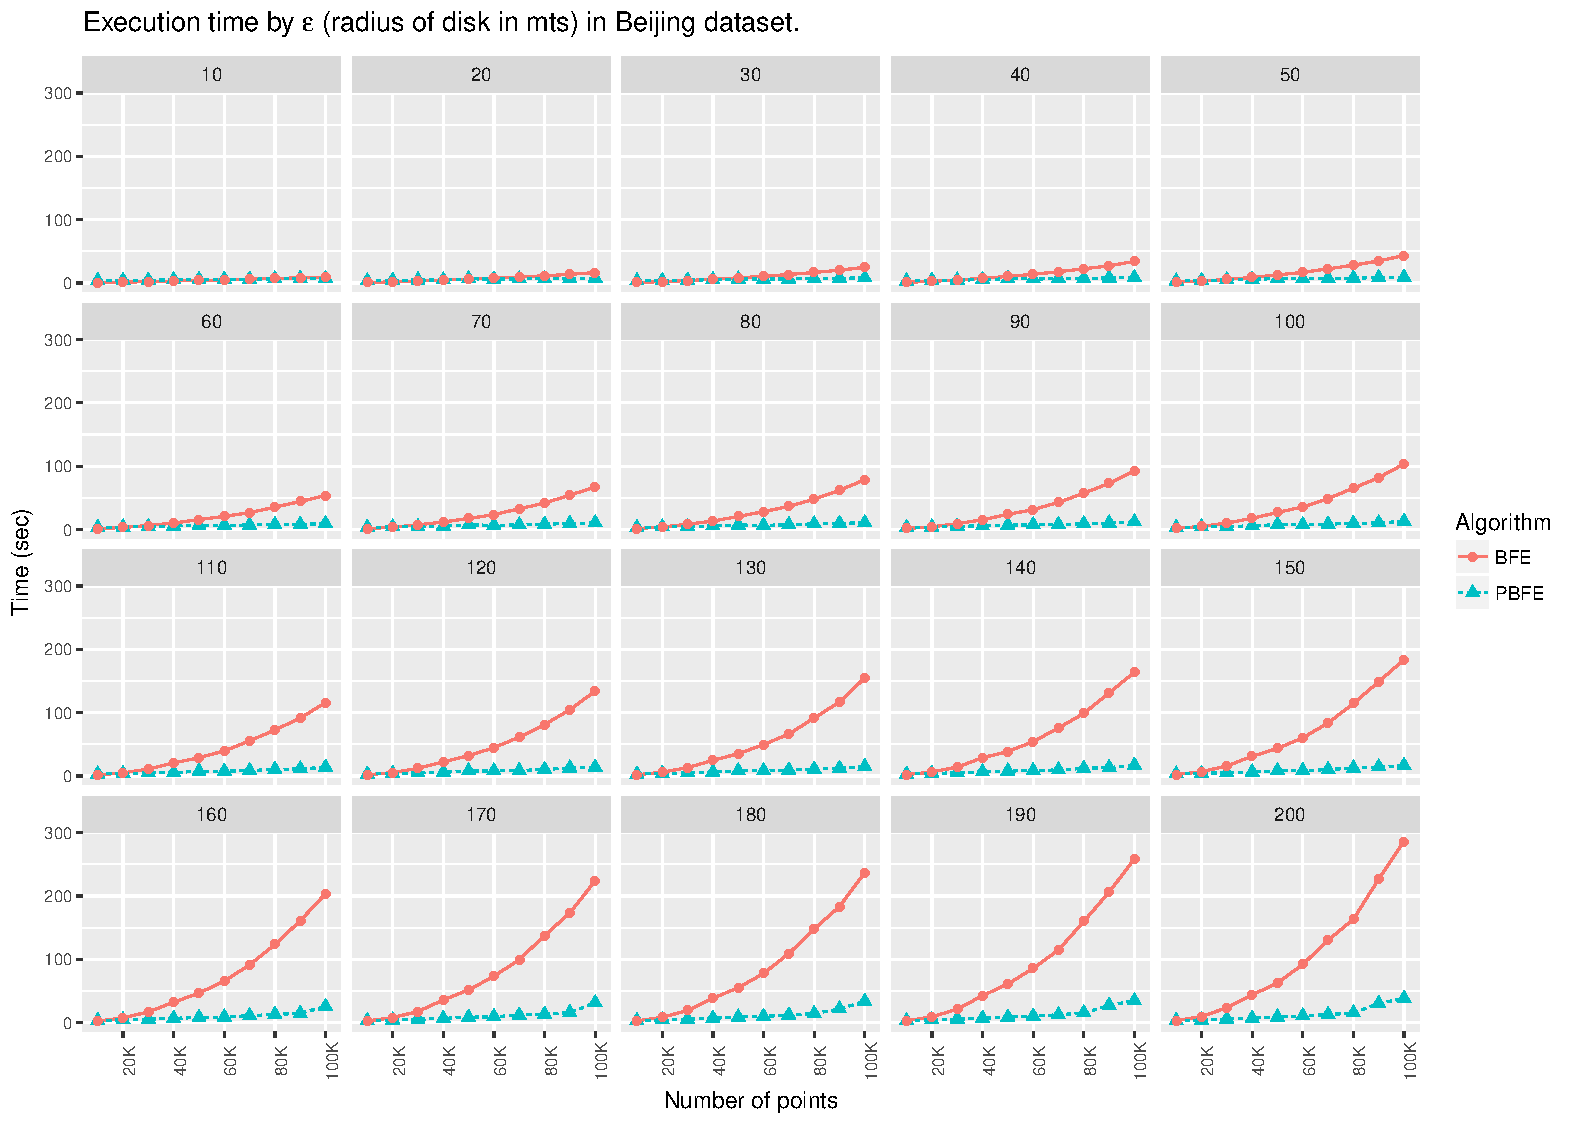
\includegraphics[width=0.9\textwidth]{figures/beijing} 
 \caption{Execution time for Beijing dataset.}
 \label{fig:beijing}
\end{figure}

\subsection{Porto dataset}
This dataset was extracted from the ECML/PKDD'15 Taxi Trajectory Prediction Challenge\footnote{\url{https://www.kaggle.com/c/pkdd-15-predict-taxi-service-trajectory-i/data}} \citep{lam_blue_2015, moreira-matias_predicting_2013}.  It collects a complete year (from 01/07/2013 to 30/06/2014) of trajectories for all the 442 taxis running in the city of Porto, in Portugal. After pre-processing and duplicate removal the collection had $\approx$17.7 million points.

This set of experiments takes data samples of 1, 2, 4, 8 and 16 million of points.  Similarly, it runs the algorithms under different values of $\varepsilon$.  This time, experiments were deployed in a 4-node academic cluster with the following setup: an 8-core Intel(R) Xeon(R) CPU E3-1230 V2 @ 3.30GHz processor and 15.5 GB of RAM per node.  The systems run Centos 6.8, Python 3.5 and Simba/Spark 1.6.0.  Figure \ref{fig:porto} show the results of these experiments.

\begin{figure}
 \centering
 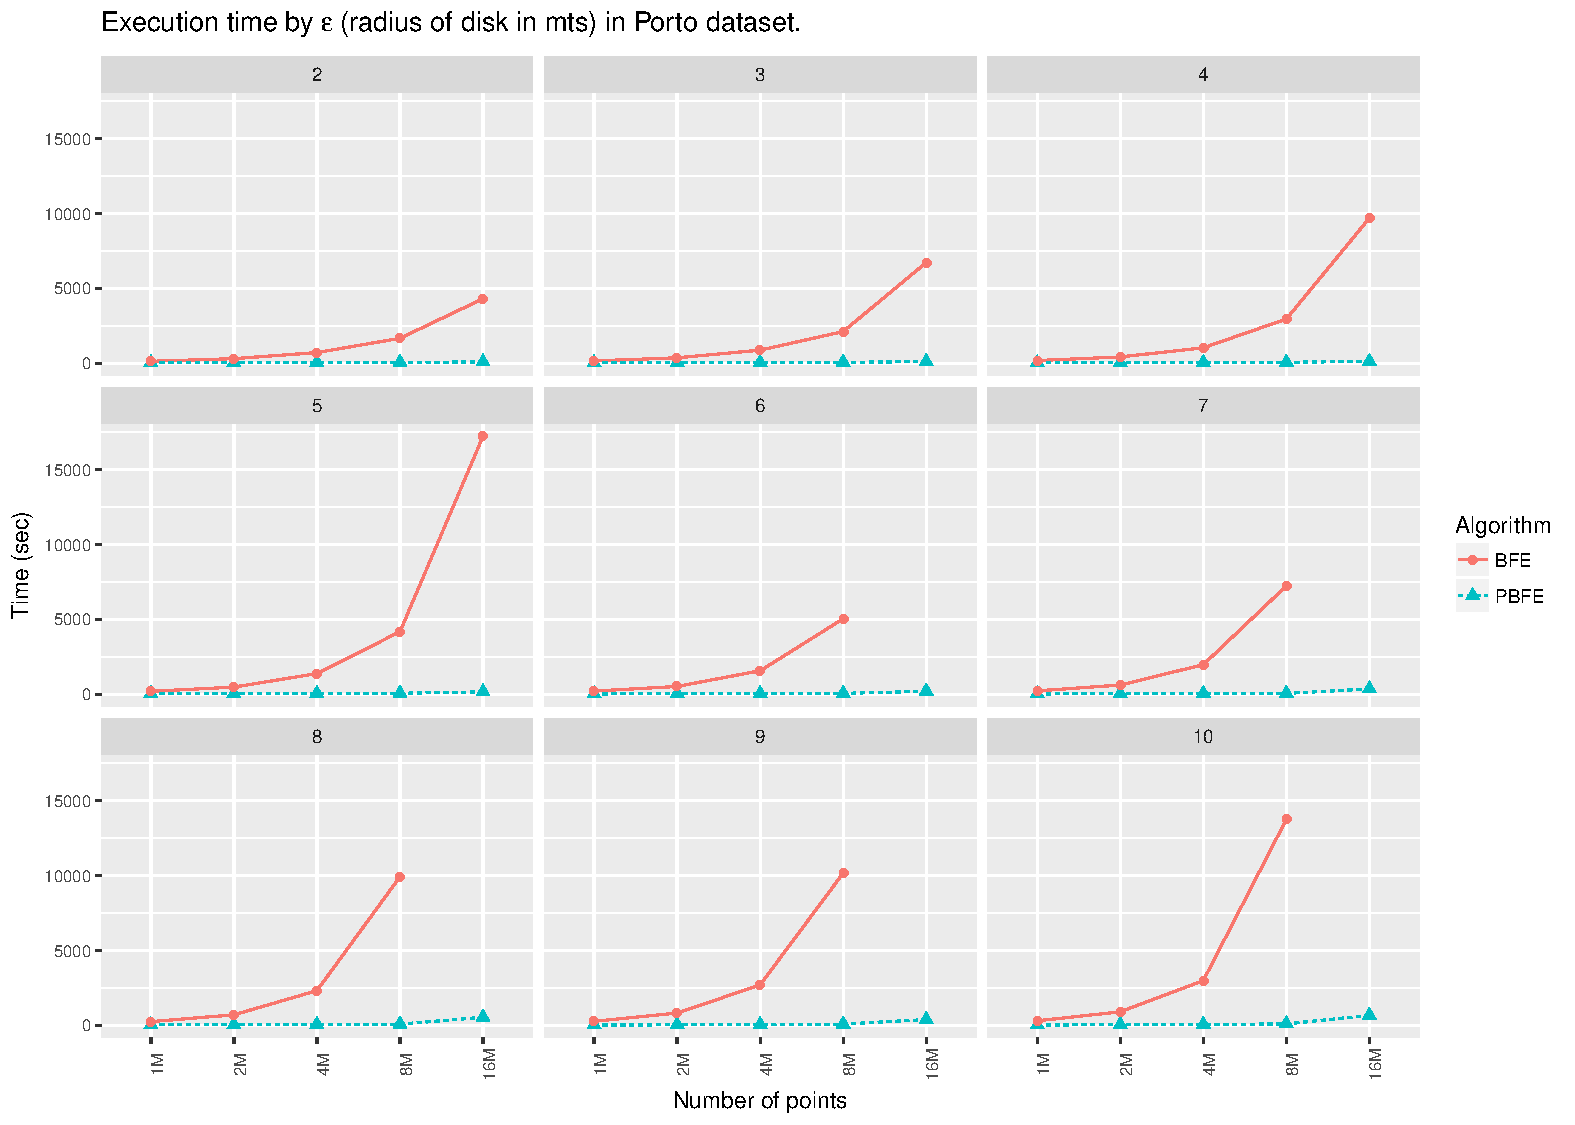
\includegraphics[width=0.9\textwidth]{figures/porto} 
 \caption{Execution time for Porto dataset.}
 \label{fig:porto}
\end{figure}

\subsection{Cologne dataset}
The SUMO (Simulation of Urbar MObility) project \citep{SUMO2012} is an open source highly configurable road traffic simulator created by the Institute of Transportation Systems in the German Aerospace Center.  The project had designed a simulation scenario describing a whole-day traffic in the city of Cologne (Germany).  The data demand comes from TAPAS, a system which compute mobility wished based on information about traveling habits of Germans and the infrastructure in the area where they live\footnote{\url{http://sumo.dlr.de/wiki/Data/Scenarios/TAPASCologne}}.

The scenario was used to built a dataset collecting timestamps and location of the involved vehicles.  Data samples of 8, 10, 12, 14 and 16 million points were taken to run similar experiments as described in the previous section. Figure \ref{fig:cologne} show the results of these experiments.

\begin{figure}
 \centering
 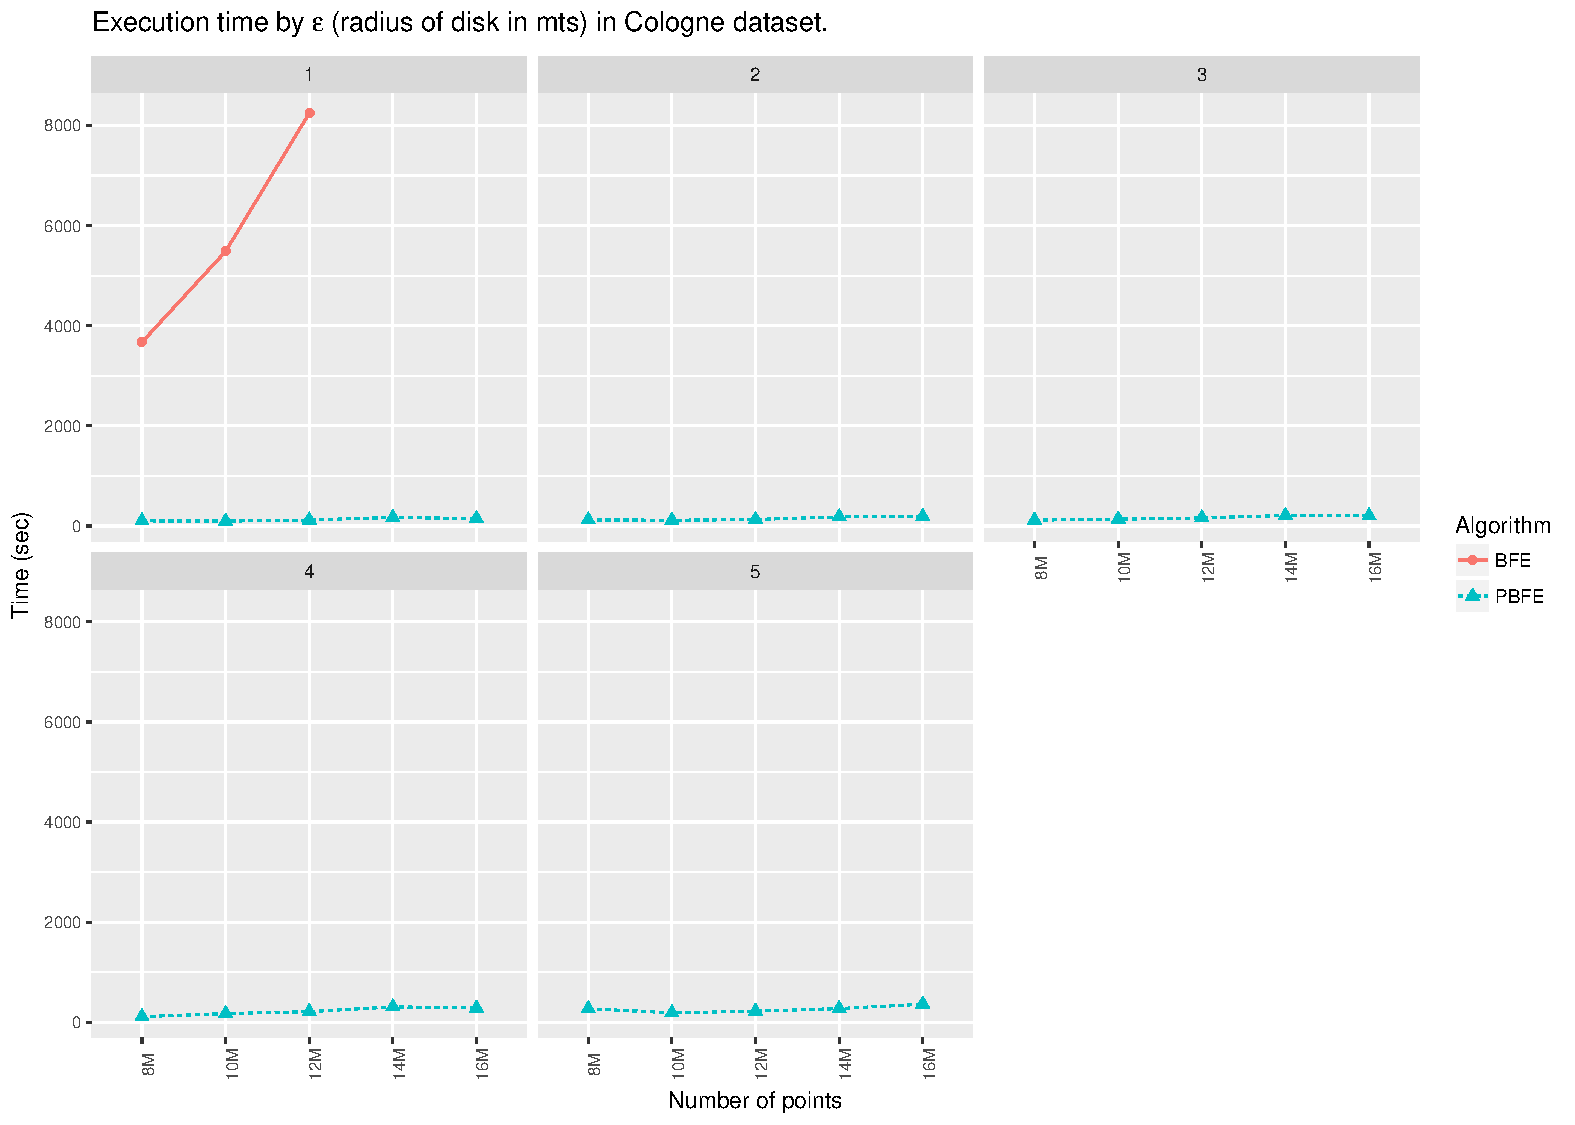
\includegraphics[width=0.9\textwidth]{figures/cologne} 
 \caption{Execution time for Cologne dataset.}
 \label{fig:cologne}
\end{figure}

\subsection{Speedup and Scaleup}
In order to test the scalability and parallel performance of our implementation, the speedup and scaleup metrics were applied to measure the improvement of the algorithm when more resources are added to the cluster.  The following experiments show speedup and scaleup of the implementation comparing the execution using just one core and after the addition of more nodes to the cluster (each node add 8 new cores).  Figures \ref{fig:SSBeijing}, \ref{fig:SSPorto} and \ref{fig:SSCologne} show the results for each of the studied datasets using different values for $\varepsilon$.

\begin{figure}
\centering
\begin{subfigure}{.5\textwidth}
  \centering 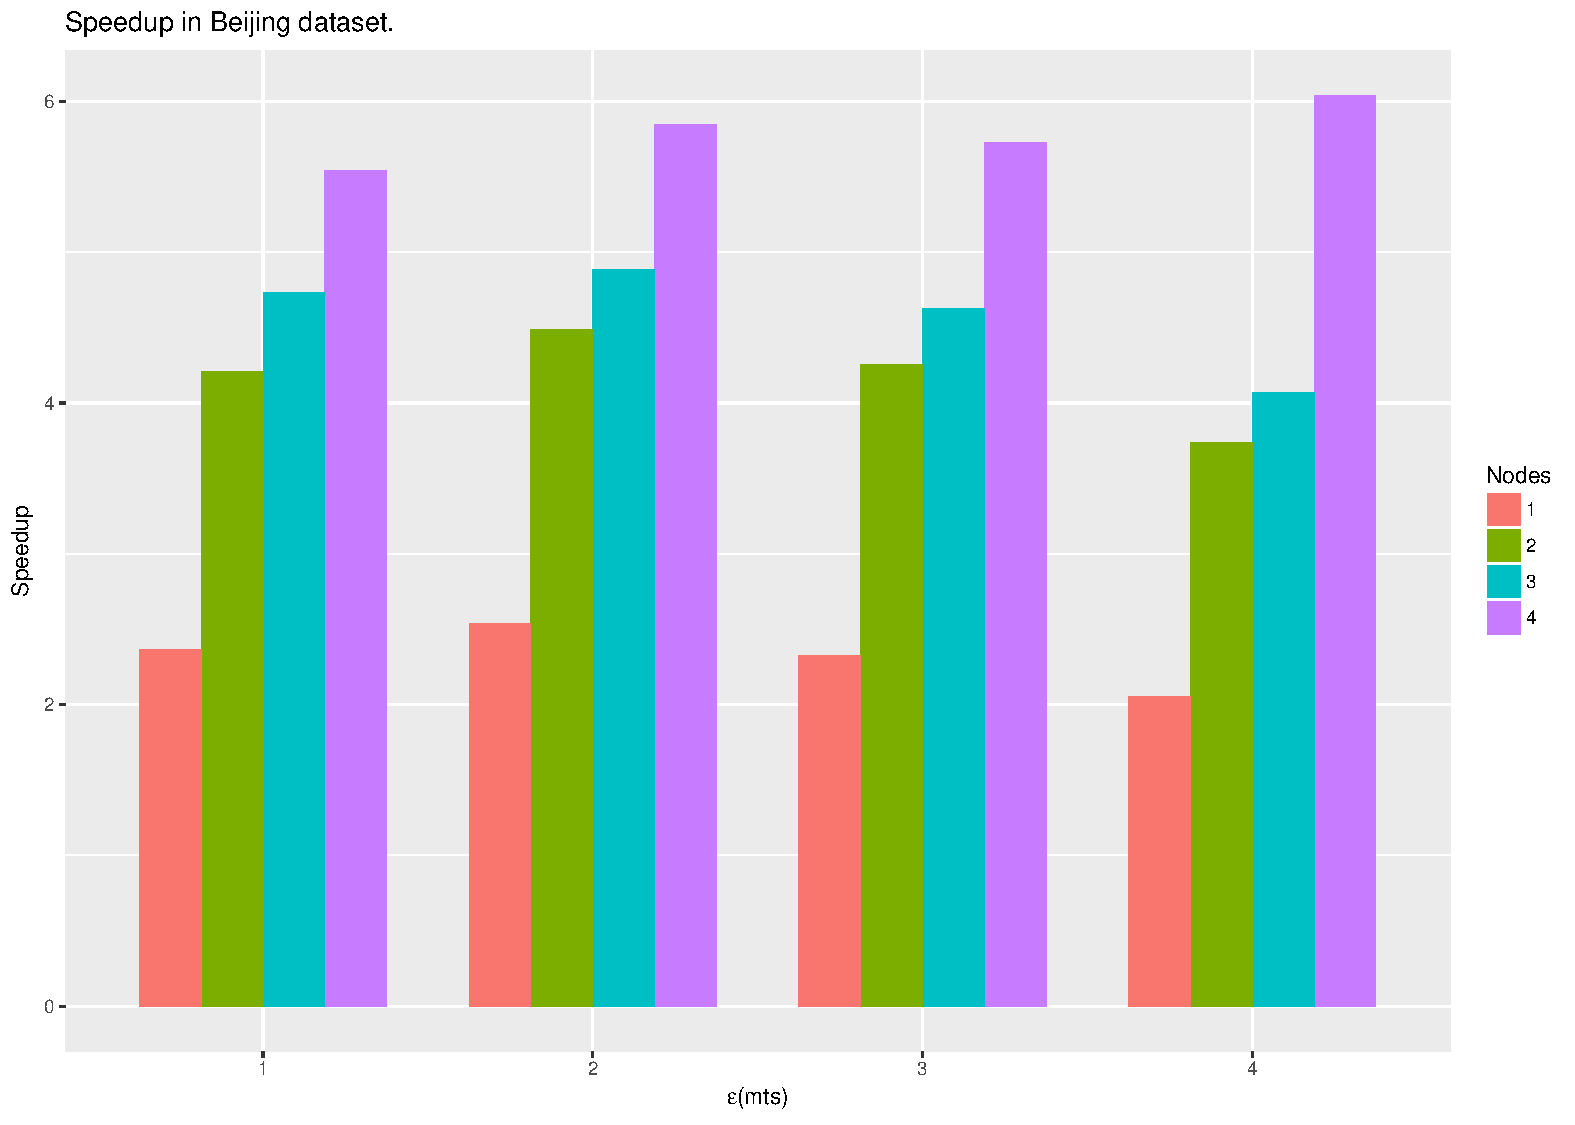
\includegraphics[width=\linewidth]{figures/2_Beijing_Speedup}
\end{subfigure}%
\begin{subfigure}{.5\textwidth}
  \centering 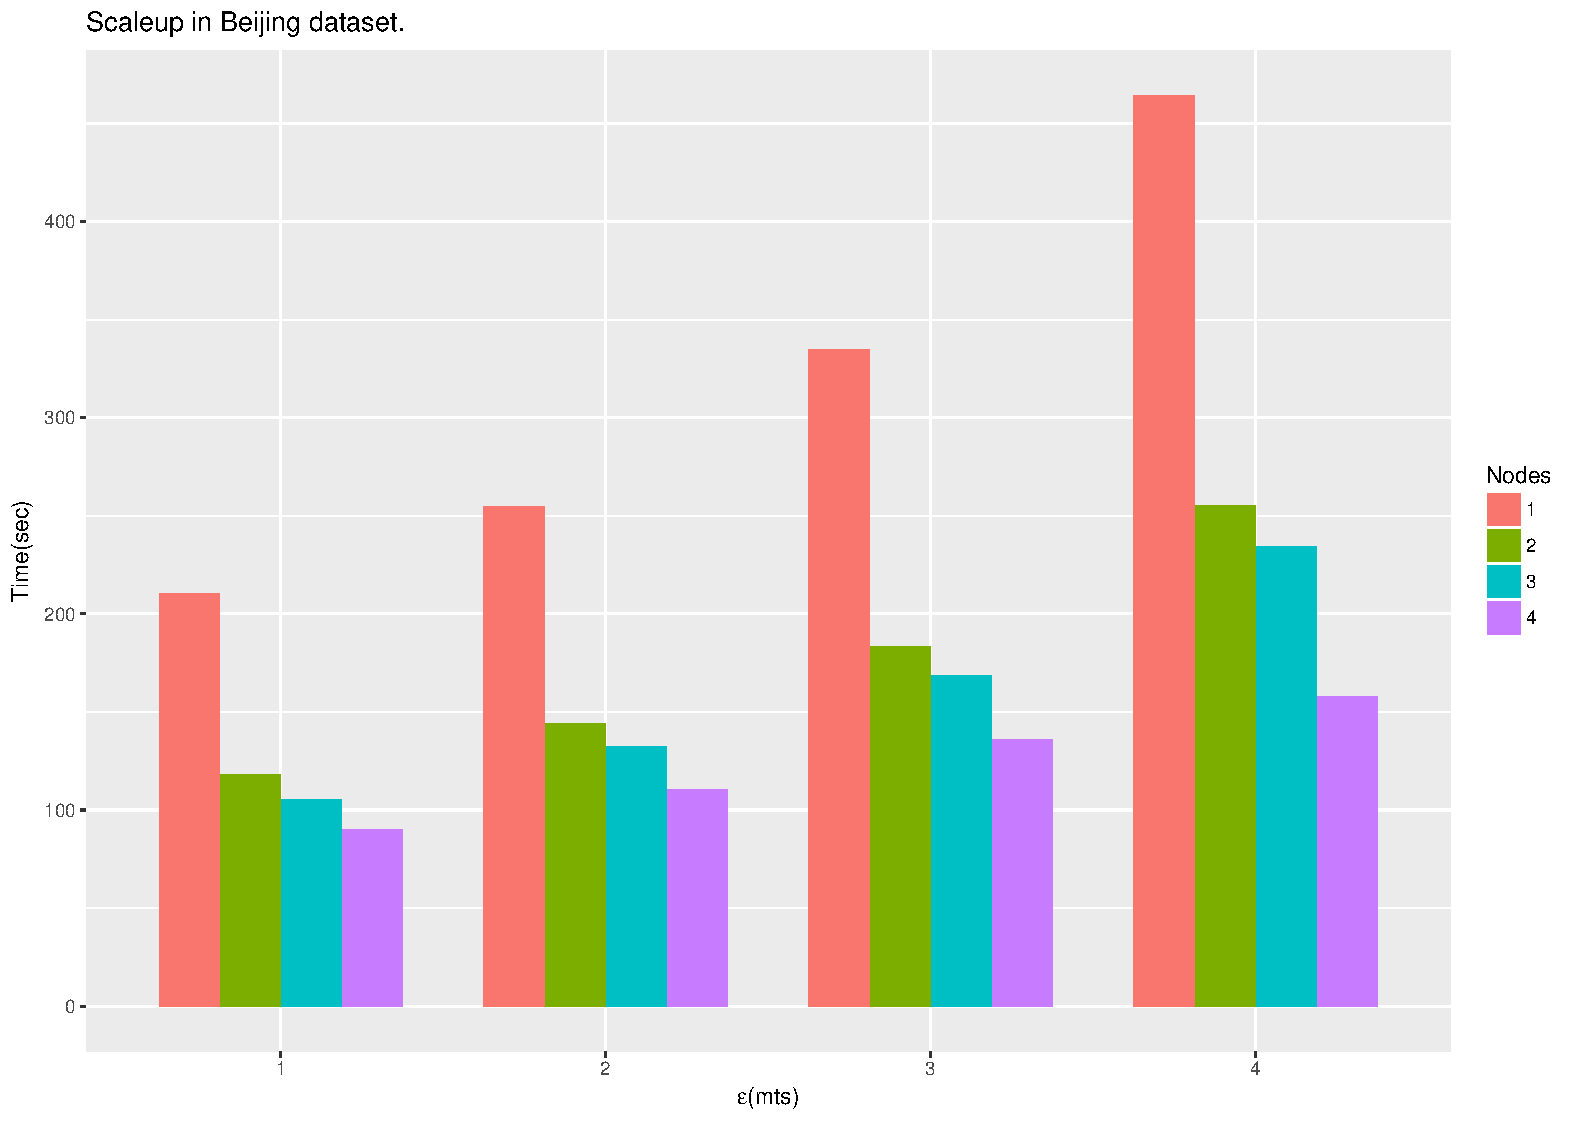
\includegraphics[width=\linewidth]{figures/3_Beijing_Scaleup}
\end{subfigure}
\caption{Speedup and Scaleup in Beijing dataset.}
\label{fig:SSBeijing}
\end{figure}

\begin{figure}
\centering
\begin{subfigure}{.5\textwidth}
  \centering 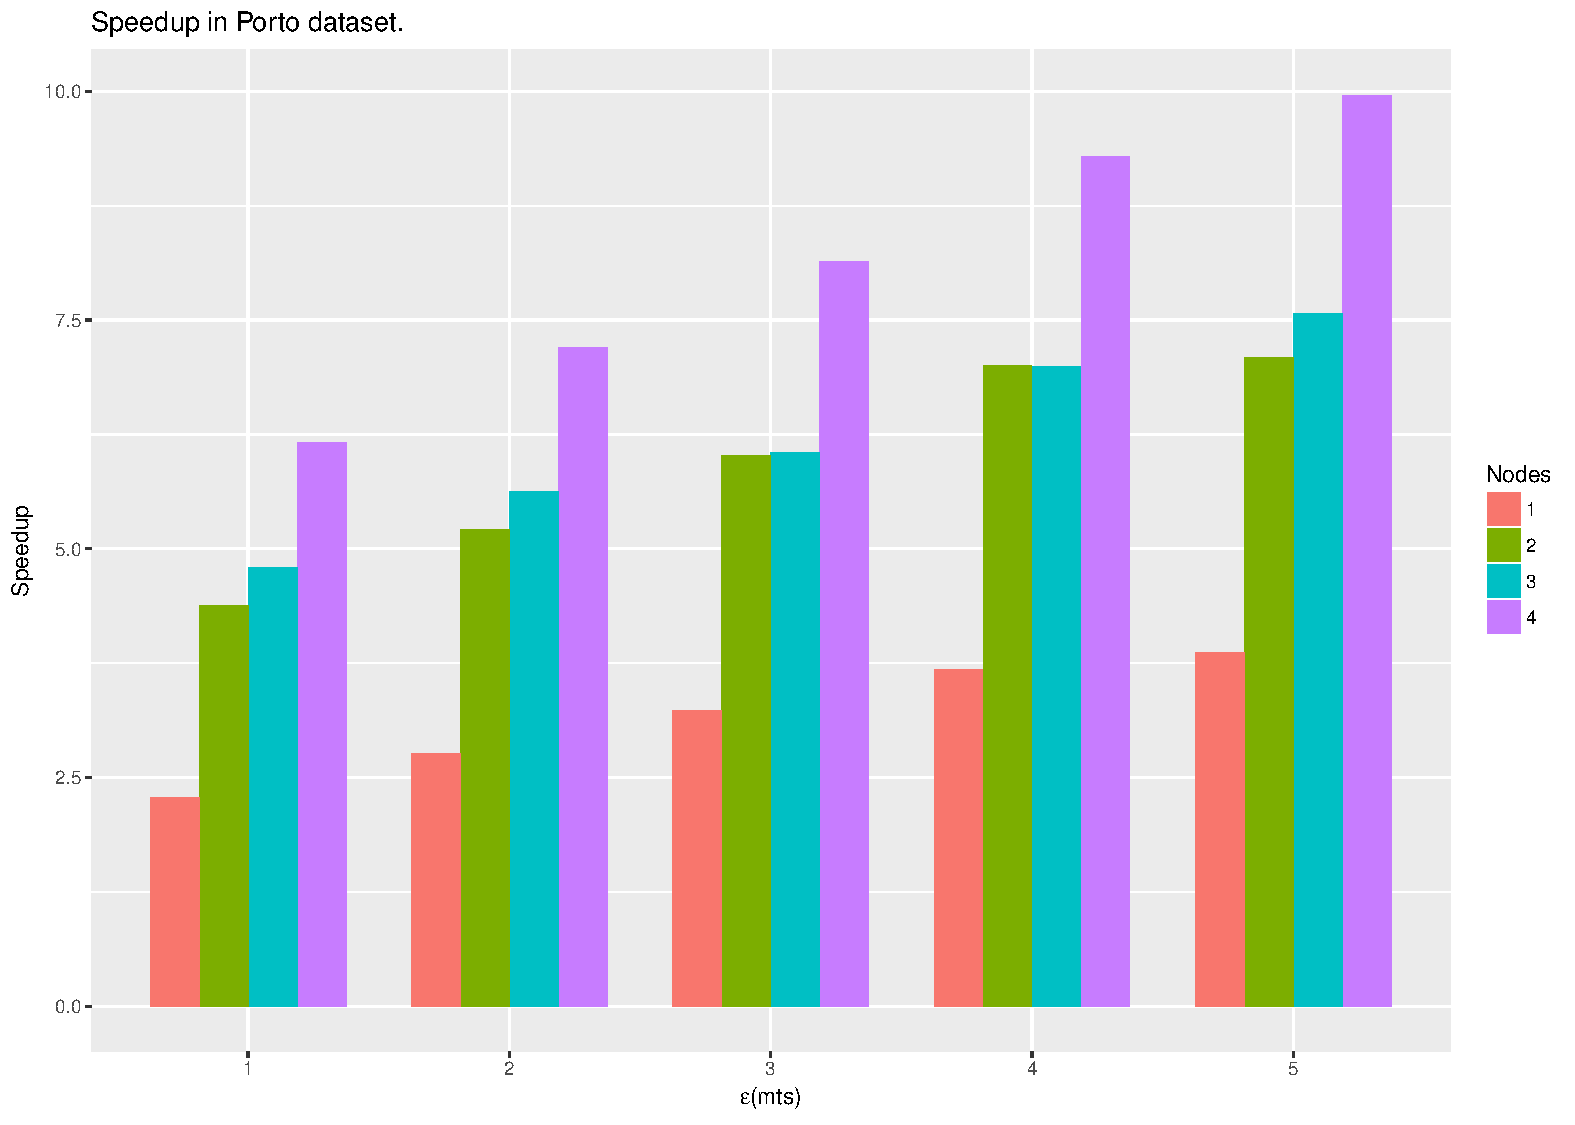
\includegraphics[width=\linewidth]{figures/2_Porto_Speedup}
\end{subfigure}%
\begin{subfigure}{.5\textwidth}
  \centering 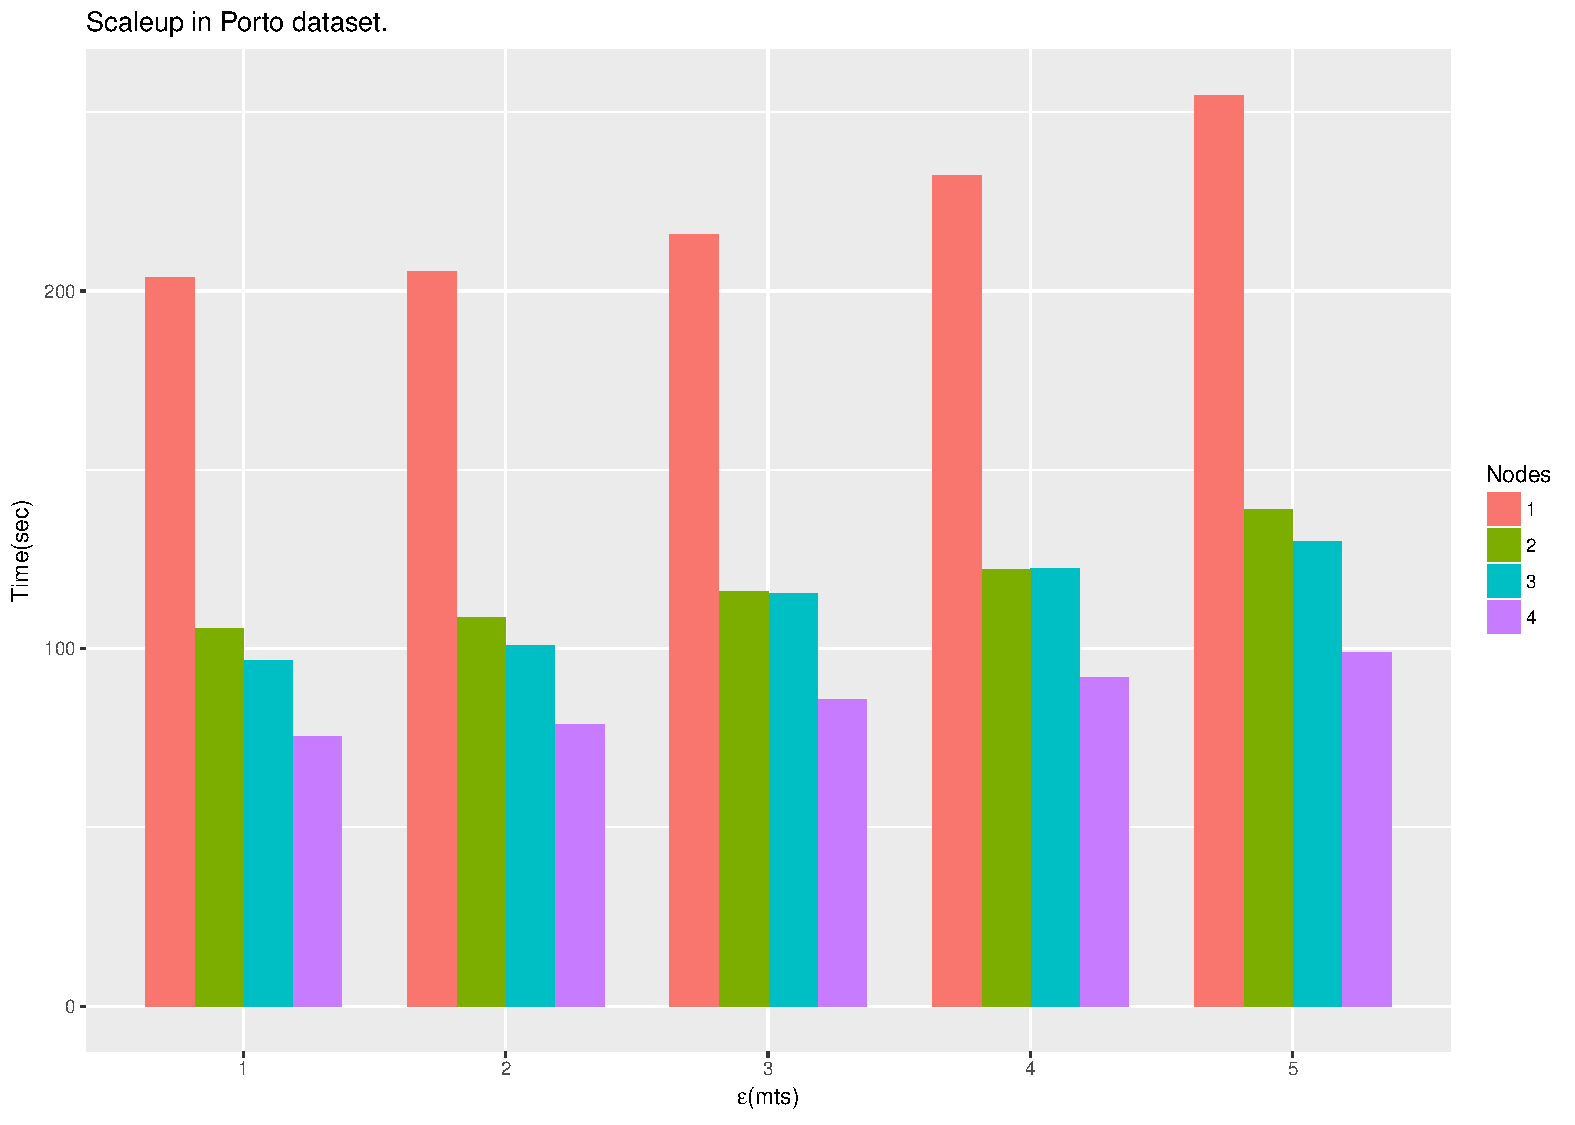
\includegraphics[width=\linewidth]{figures/3_Porto_Scaleup}
\end{subfigure}
\caption{Speedup and Scaleup in Porto dataset.}
\label{fig:SSPorto}
\end{figure}

\begin{figure}
\centering
\begin{subfigure}{.5\textwidth}
  \centering 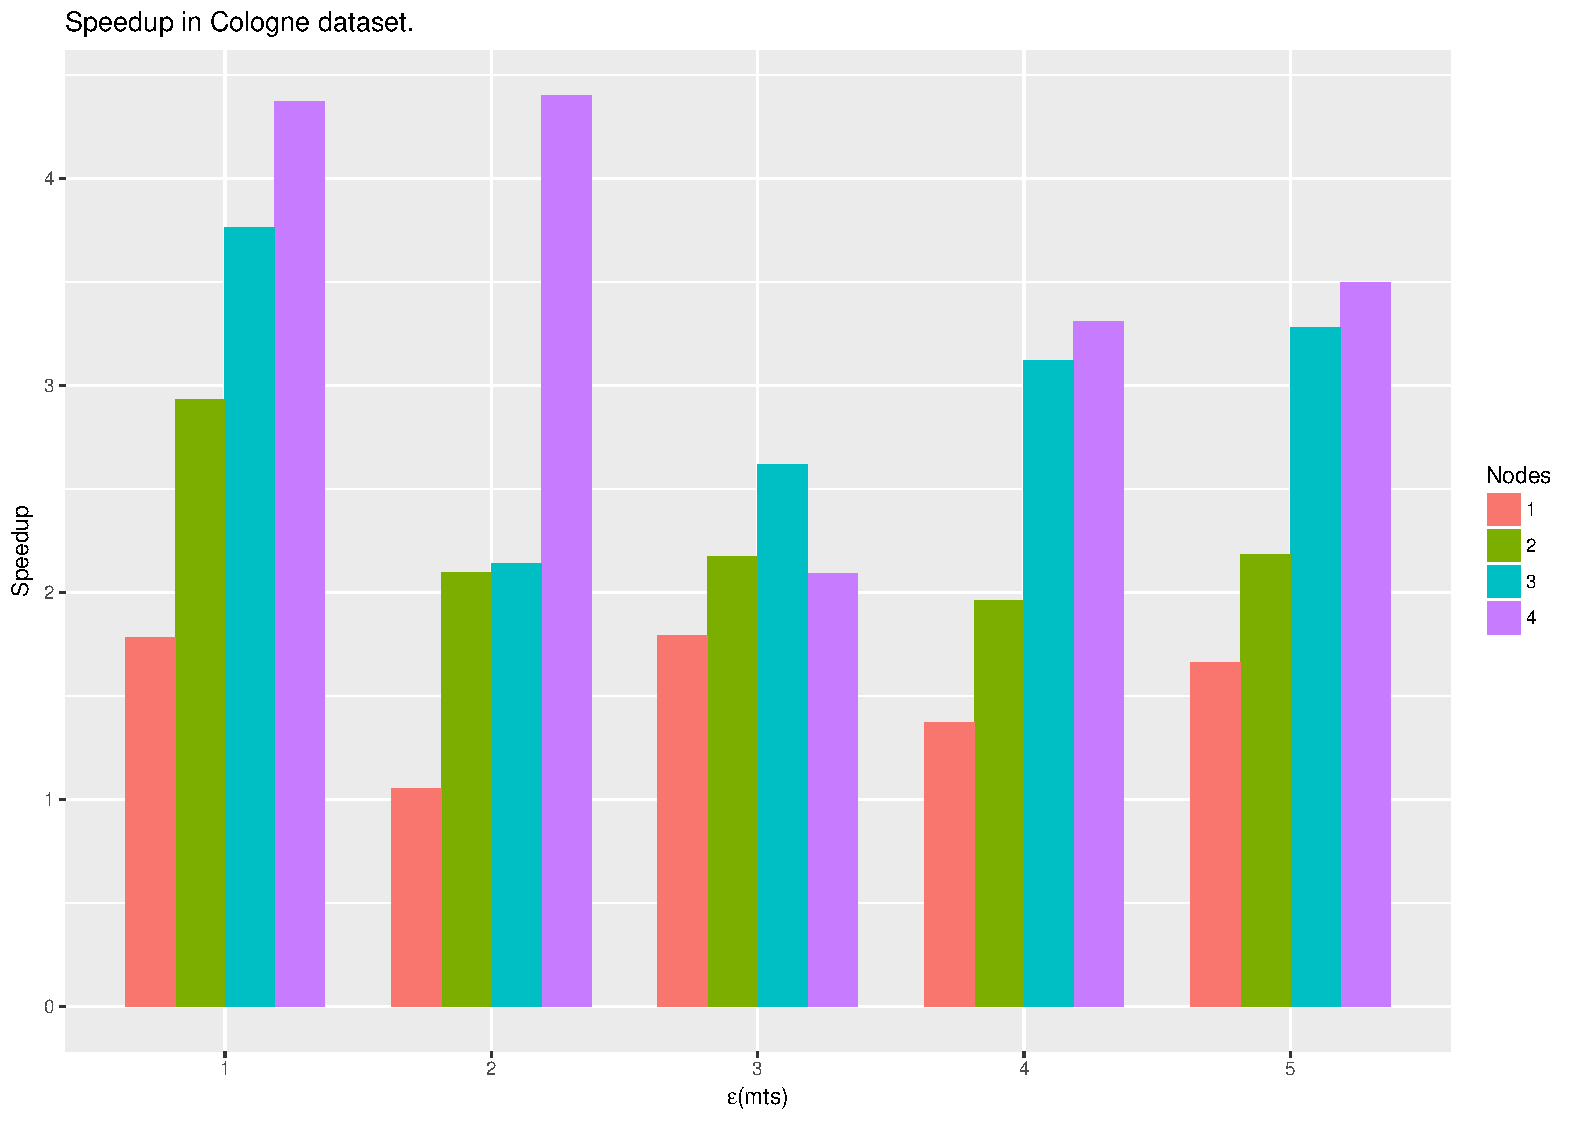
\includegraphics[width=\linewidth]{figures/2_Cologne_Speedup}
\end{subfigure}%
\begin{subfigure}{.5\textwidth}
  \centering 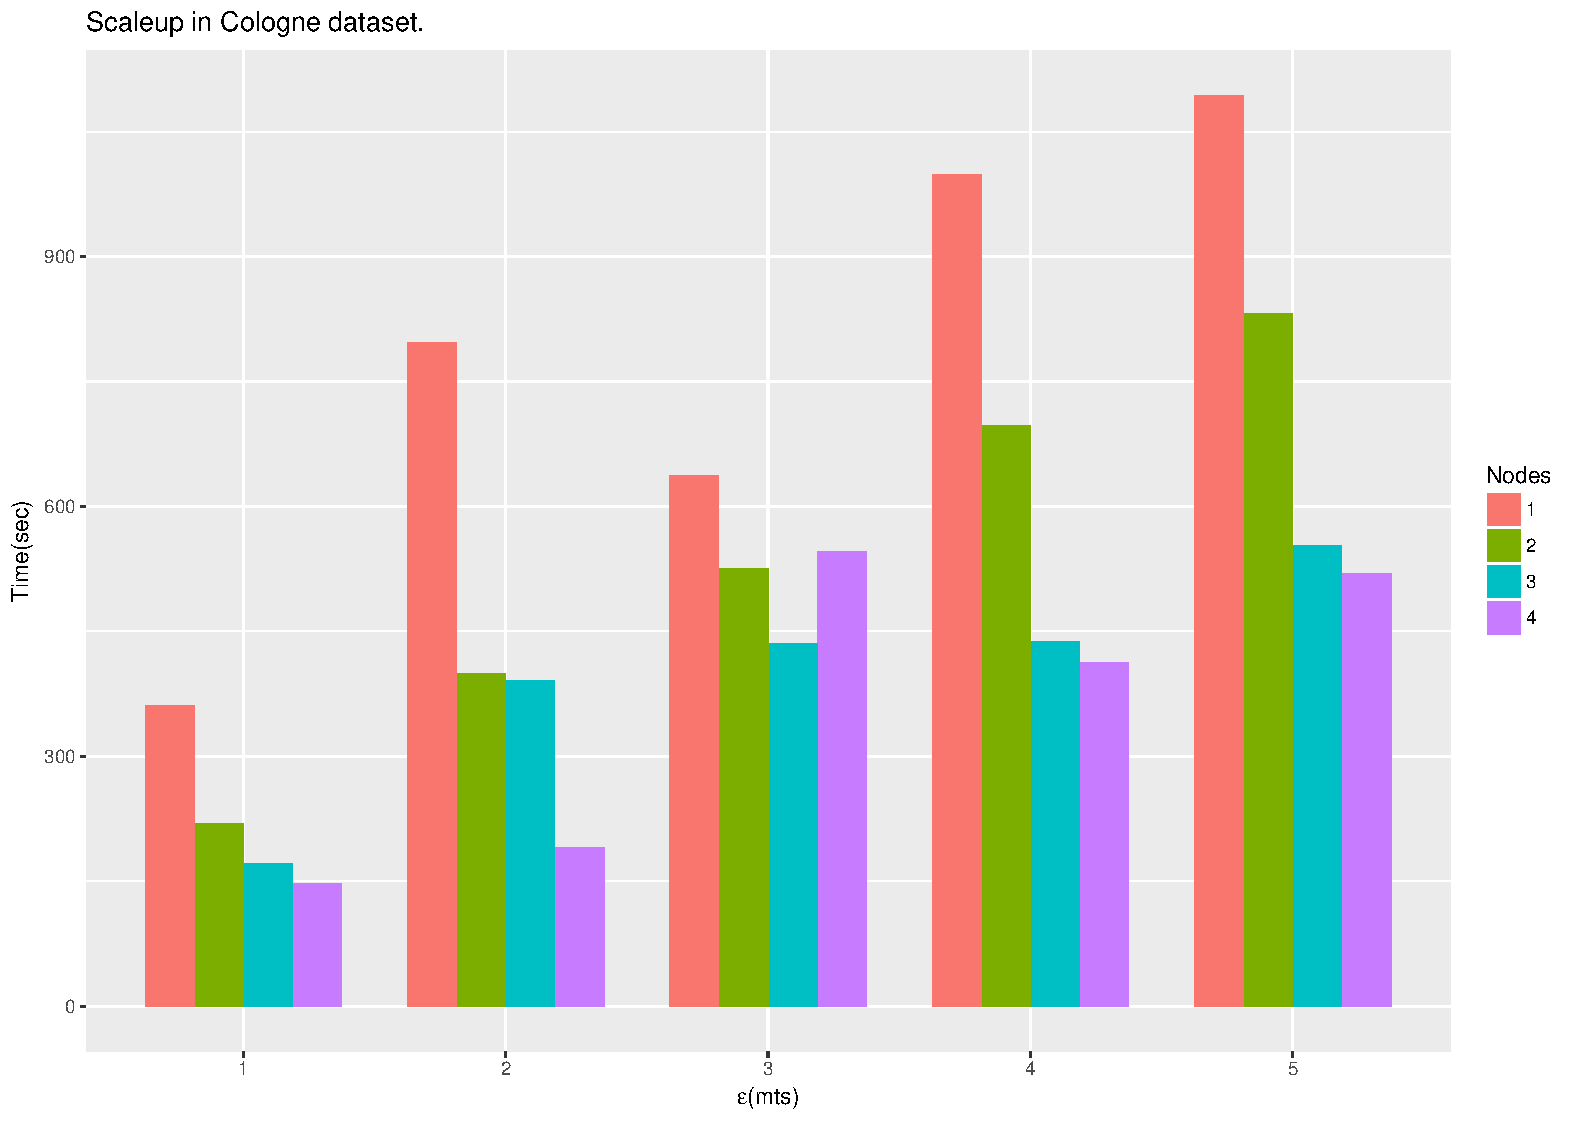
\includegraphics[width=\linewidth]{figures/3_Cologne_Scaleup}
\end{subfigure}
\caption{Speedup and Scaleup in Cologne dataset.}
\label{fig:SSCologne}
\end{figure}

\section{Finding maximal set of disks}
Section \ref{sec:candidates} explains how to find a valid set of candidates disks but it is not a final set.  Many of the disks are redundant (they are contained by others) or they do not contain the minimum number of requested objects ($\mu$ parameter).  The final set of valid disks is known as the set of maximal disks.  BFE faces the issue through an iterative filter over all the candidate disks discarding those whose do not fulfill the requirements by direct comparison. However, it can be a costly operation according with the number of disks.

For this stage, we propose apply a frequent pattern mining approach to filter the candidate disks.  The main idea is to filter redundant disks by applying well-known frequent pattern algorithm for maximal pattern detection \citep{Han:2005:DMC:1076797}.

Maximal patterns are valid representation of the complete set of frequent patterns for a dataset because they contains all the subsets whose overpass a minimum threshold.  They are important because all the remaining frequent patterns can be computed from them.  Many efforts and techniques have been developed in order to find efficient methods to find this particular kind of patterns.  

\cite{fimi03_report} and \cite{Fournier-Viger2016} have explored and collected a significant number of implementations and details about the available algorithms in the topic.  Among the available techniques, \cite{uno_lcm_2004} propose the LCM algorithm which stands out as one of the most efficient implementation. It is able to find maximal sets in linear time according with the number of patterns.

Given that the maximal set of disks are those that contain redundant disks, maximal frequent patterns algorithms can be used to detect those disks.  If the objects enclosed by the disks are seen as transactions, it results simple to apply any technique to discover maximal patterns.  

\subsection{Experiments}
This section shows a set of preliminary experiments to test the suitability of using a frequent pattern mining approach to find the set of maximal disks.  The main idea is to collect the objects enclosed by the candidate disks as transactions and built a dataset which will be evaluated by a maximal frequent pattern algorithm (LCM in this case).

To parallelize the algorithm, a local-global approach was used.  In this case, the transaction version of the candidate set was distributed among the available nodes and LCM was run over the local datasets.  In a global step, the results were merged in a unique dataset and a final run on LCM was executed on it.  The main advantage was that each local run of LCM return a much smaller dataset which can be processed in linear time.

The experiments use reduced samples of Beijing and Porto datasets as described in section \ref{sec:experiments}.  The setup is also similar to that used in the Porto and Cologne experiments.  Figures \ref{fig:mbeijing} and \ref{fig:mporto} shows the results.

\begin{figure}
 \centering
 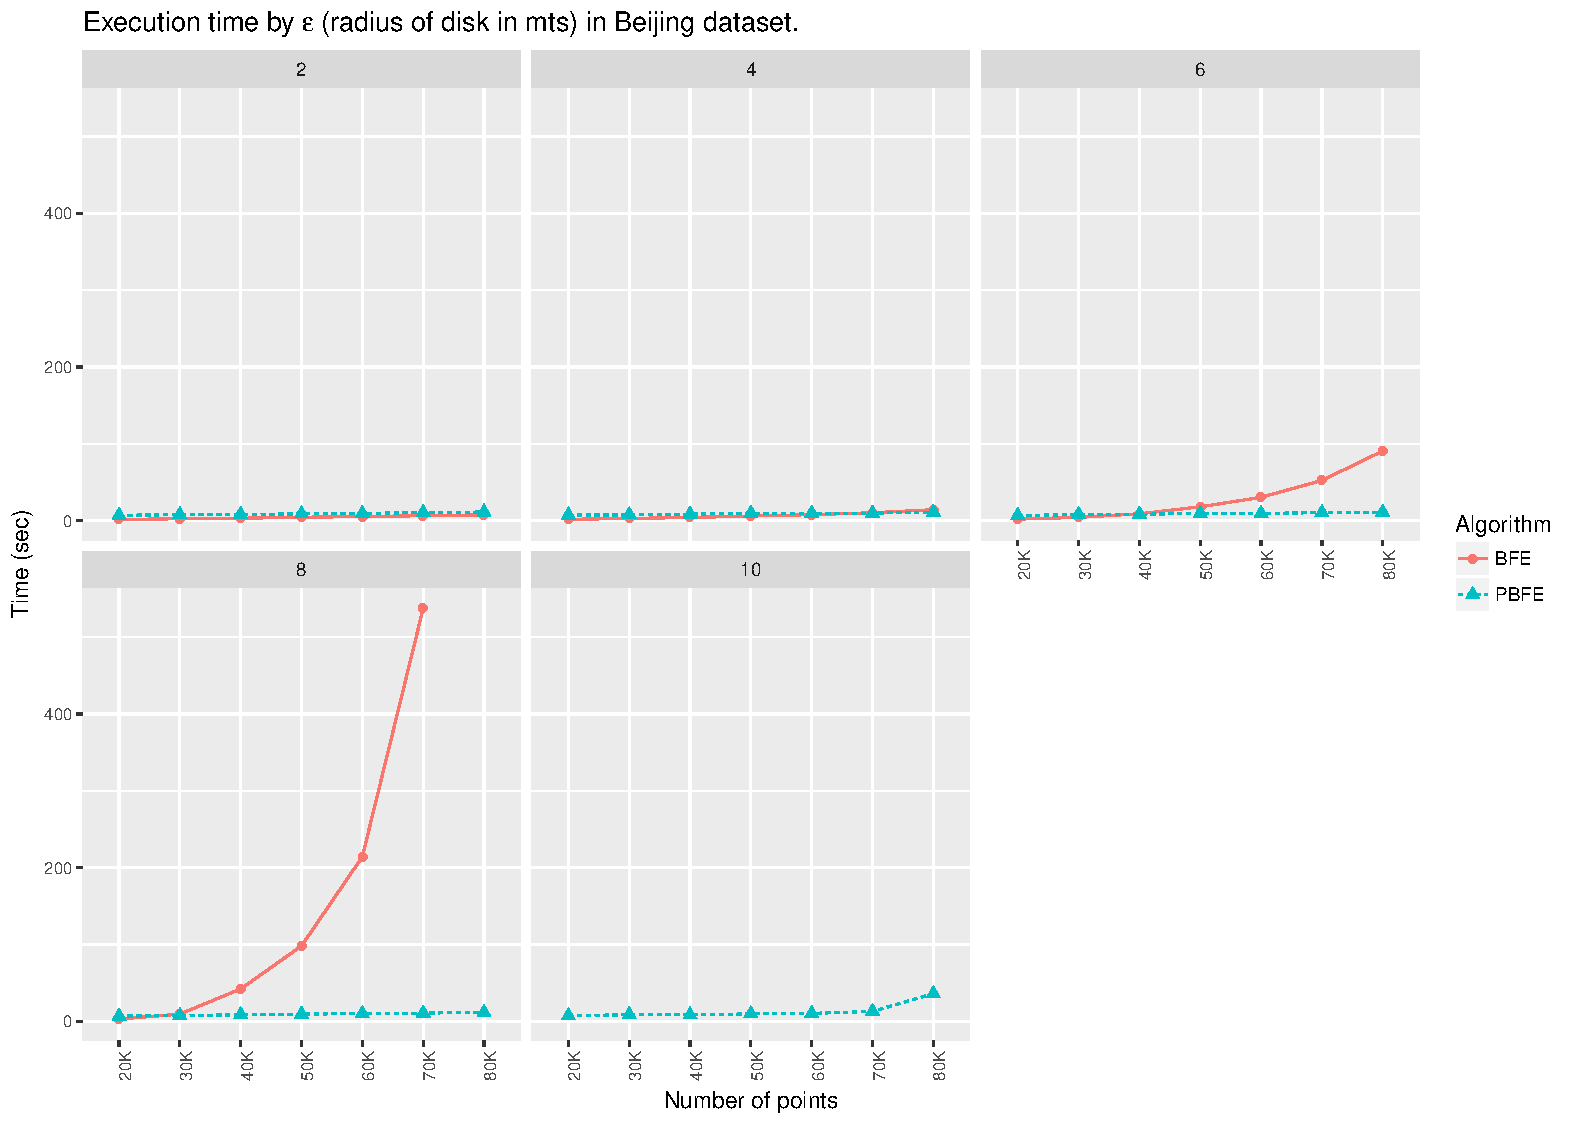
\includegraphics[width=0.9\textwidth]{figures/mbeijing} 
 \caption{Execution time for Beijing dataset.}
 \label{fig:mbeijing}
\end{figure}

\begin{figure}
 \centering
 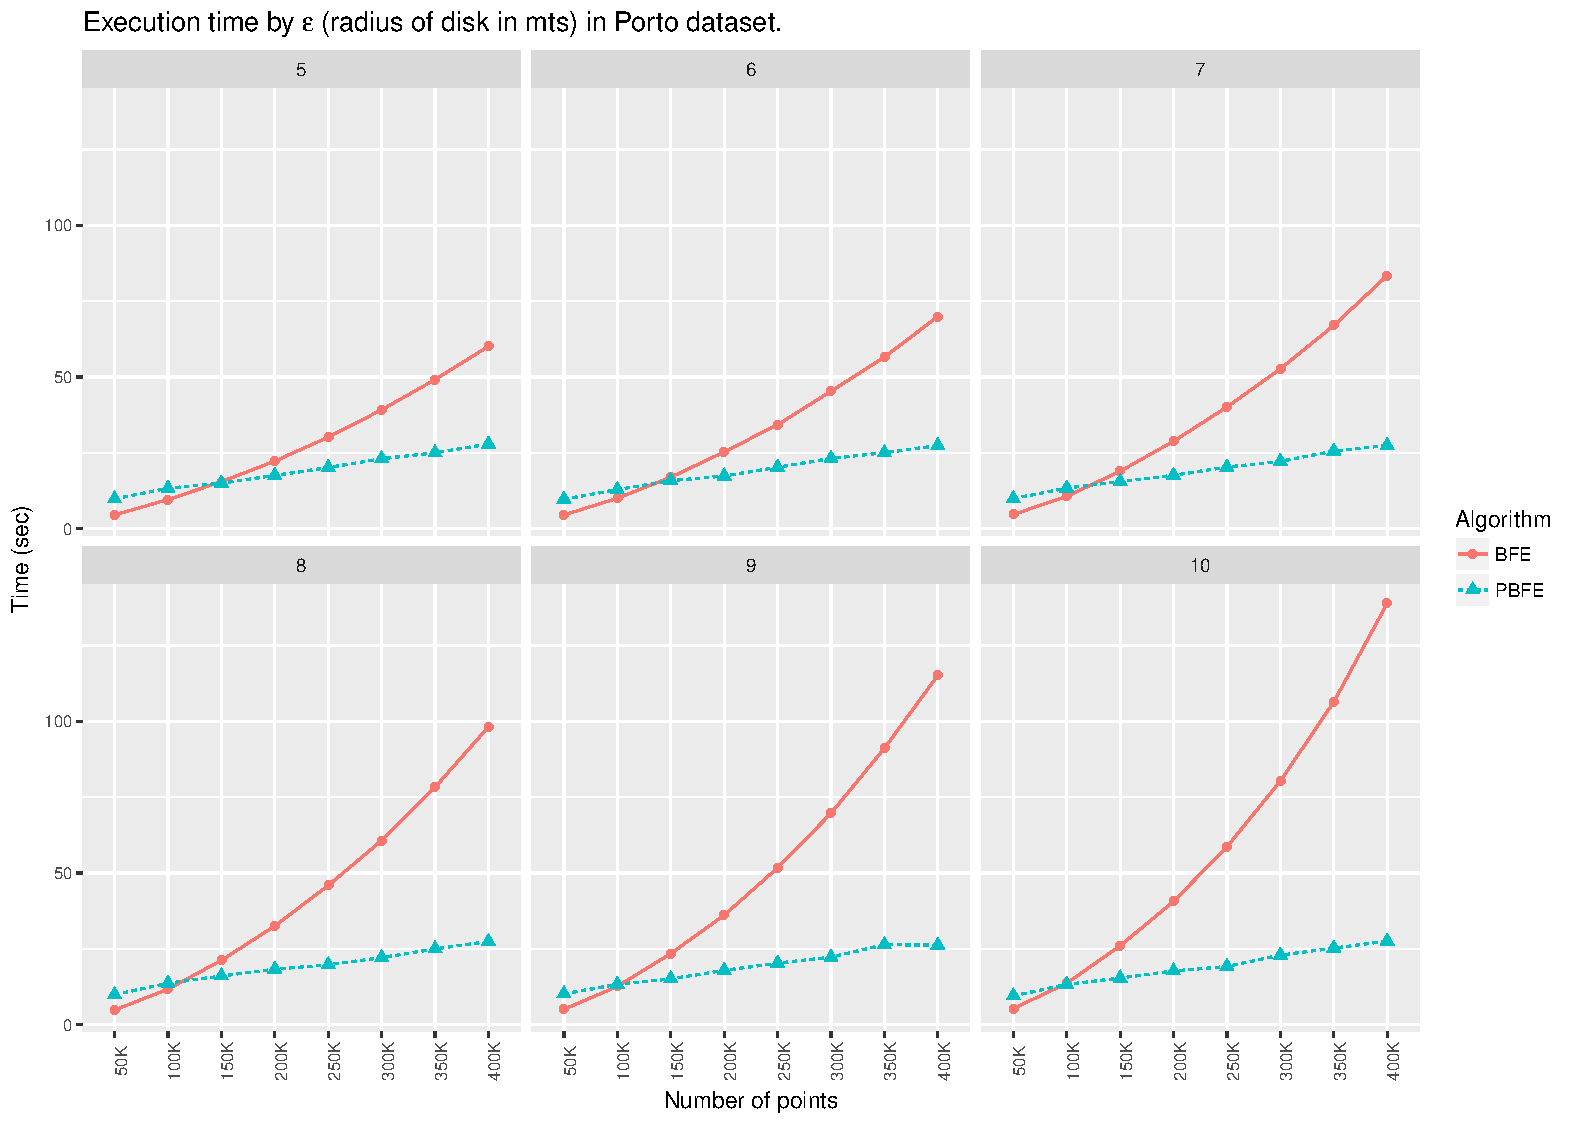
\includegraphics[width=0.9\textwidth]{figures/mporto} 
 \caption{Execution time for Porto dataset.}
 \label{fig:mporto}
\end{figure}

\section{Conclusions and future work}\label{sec:conclusions}

An implementation of a parallel method to detect disks for the BFE algorithm has been presented.  The proposed method proves to be scalable and reliable. Experiments shows that execution time improves up to 3 orders of magnitude compared to the sequential implementation of the BFE algorithm for the same step.

Parallel implementation for the remaining steps of the BFE algorithm are part of the future work. It is expected to work on a parallel strategy to join the sets of valid disks between time intervals.  Also, others approaches for partitioning should be explored, especially in the case of finding maximal disks.  The local-global approach is just a preliminary prototype. Certainly, a proper parallel implementation of LCM algorithm should be an interesting idea. In addition, data pre-processing and result visualization are still open issues.

\bibliographystyle{plainnat}
\bibliography{flock}

\end{document}
